\documentclass{article}

\usepackage{arxiv}
\usepackage{amsmath, amsfonts, amssymb}
\usepackage{graphicx}
\usepackage{hyperref}
\usepackage{booktabs}
\usepackage{enumitem}
\usepackage{float}
\usepackage{tikz}
\usetikzlibrary{arrows.meta, positioning, shapes.geometric, calc, fit}
\setlength{\headheight}{23pt}
\makeatletter
\def\headeright{}
\def\undertitle{}
\makeatother
\AtBeginDocument{
  \setlength{\headheight}{23pt}
  \addtolength{\topmargin}{-9pt}
}

\title{Stewardship Harnesses:\\
Maintaining Executable Intelligence Across Agent Loops}

\author{
  Josh Rosen \\
  ThruWire, Inc.
  \And
  Seth Rosen \\
  ThruWire, Inc.
}

\begin{document}

\maketitle

\begin{abstract}
Multi-agent AI systems are increasingly organized as collections of looping agents that plan, call tools, delegate work, and produce local outputs. Interoperability protocols help such agents discover one another, advertise capabilities, and exchange tasks or artifacts. Yet communication alone does not solve a deeper systems problem: each outer loop is usually optimized to complete the task in front of it, not to preserve and improve the shared structure future agents will inherit. As many locally successful agents operate over time, they can accumulate cross-agent drift: stale assumptions, inconsistent intermediate artifacts, duplicated procedures, incompatible context-selection practices, and final outputs that no longer agree with maintained upstream state.

We hypothesize that long-lived, dependency-bearing multi-agent systems need outer loops to act as stewards of shared executable intelligence. By \emph{executable intelligence}, we mean durable, versioned procedures and artifacts that future agents can run against: context patterns, artifact contracts, current-state resolution rules, dependency structure, validation gates, and affectedness semantics. An outer loop is not merely a task solver or message participant. It is also a consumer of shared structure: when a task matches an existing procedure, the loop should ask the shared harness to execute that structure with task-specific inputs and parameters, consume the resulting artifacts or context bundle, and publish through existing artifact contracts. When the task reveals a gap, the loop should improve the shared structure future agents will inherit.

A shared stewardship harness is an MCP-accessible execution control plane that maintains dependency-aware artifacts, executable context patterns, supersession semantics, current-state resolution, and propagation rules. A context pattern is not merely a prompt template or retrieval query; it is an executable procedure that determines which artifacts, inputs, slots, constraints, and generated intermediates should be loaded, omitted, generated, or refreshed for a class of task. The harness makes these patterns durable and improvable, while outer loops are responsible for observing when a pattern is incomplete, overloaded, stale, or reusable in a stronger form.

The contribution is a systems abstraction and reference architecture rather than an empirical benchmark. We distinguish agent interoperability from maintained intelligence, define the stewardship harness and executable context patterns, describe how MCP-mediated outer loops can execute against existing structure and improve it after acting, and outline evaluation criteria for future work. The central architectural claim is that some multi-agent systems need not only better ways for agents to talk, but explicit mechanisms for maintaining the executable shared state that future loops inherit. Whether such mechanisms reduce drift or improve downstream work is an empirical question for future evaluation.
\end{abstract}

\section{Introduction}

Outer agent loops are effective local problem solvers. A coding agent can inspect a repository, patch files, run tests, and report a result. A research agent can gather sources, synthesize a memo, and hand off an answer. A planning agent can decompose a goal, call tools, and delegate subtasks. These loops are useful because they are flexible: they can explore, recover from partial failure, revise plans, and adapt to the task in front of them \cite{yao2023react,schick2023toolformer,wu2023autogen,li2023camel,hong2023metagpt,wang2023voyager}.

The same flexibility becomes a systems problem when many loops operate over long-lived shared work. Each outer loop is commonly rewarded for completing its visible task, not for improving the maintained execution environment that future loops will inherit. A locally successful agent may patch a final memo while leaving the upstream criteria artifact stale. Another may invent a better analysis procedure but preserve it only in a transcript. A third may retrieve a different mixture of prior context and reach an incompatible conclusion. Across many agents, local task success can compound global drift.

We call this failure mode \emph{cross-agent drift}: loss of coherence across many loops as agents assemble different context, preserve different assumptions, update different artifacts, and leave authority unresolved. The central distinction is that agent communication is not the same as maintained executable shared state. A set of agents may exchange messages fluently while still disagreeing about which artifacts are current, which procedures should run, which outputs are stale, and which changes affect downstream work.

This paper proposes a shared stewardship harness for long-lived, dependency-bearing multi-agent systems: an MCP-accessible execution control plane that enables outer loops to maintain executable context patterns, durable intermediate artifacts, supersession semantics, current-state resolution, and dependency-aware propagation. The harness runs alongside outer agent loops as a shared coprocessor for durable responsibilities. The outer loop remains flexible, exploratory, and task-directed. The harness owns shared structure: artifact lineage, executable graph state, context-pattern registries, invalidation, replay, and current-state resolution.

Executable intelligence is the part of shared state that future agents can run against: context patterns, artifact contracts, current-state resolution rules, dependency structure, validation gates, and affectedness semantics. It differs from ordinary workflow definitions because it also includes authority semantics, supersession, dependency propagation, and context-materialization behavior learned over time. Outer loops are both consumers and stewards of this structure. When a task matches existing structure, a loop can ask the harness to execute that structure with task-specific inputs and parameters, consume the resulting artifacts or context bundle, and publish through existing artifact contracts before inventing a new local procedure. After acting, the loop should leave behind better artifacts, better context-selection procedures, better dependency structure, better validation rules, or explicit evidence that no shared update was needed.

A simple contrast makes the systems requirement concrete. A locally complete loop finishes a competitive-risk memo, notes that services-heavy companies require different criteria, and exits. A stewardship-compliant loop completes the memo, proposes a criteria-artifact update, adds a context-pattern slot for company type, marks affected downstream artifacts stale, validates that unrelated branches remain unchanged, and records why the change should be reused. Stewardship is not merely writing memory. It is maintaining the structure that future agents will execute against.

This framing builds on two earlier ThruWire papers. The first established execution lineage: explicit directed acyclic graph (DAG) structure, stable execution identities, dependency-aware replay, and the distinction between final answer quality and maintained-state quality \cite{rosen2026lineage}. The second established intermediate artifacts as first-class state: typed, structured, addressable, versioned, dependency-aware, authoritative, and consumable by downstream computation, with additive and superseding semantics \cite{rosen2026artifacts}. The present paper asks a different question: when many outer loops operate over time, what shared execution environment lets them improve the intelligence future loops inherit?

The answer is not a generic multi-agent collaboration framework. A2A-style interoperability helps agents discover one another, delegate tasks, exchange messages, and return artifacts \cite{a2a2026spec}. It is complementary, but it does not by itself define maintained artifact authority, context-pattern learning, dependency-aware invalidation, or current-state resolution. MCP provides a better interface to the shared harness because it standardizes how AI applications access external tools, resources, prompts, and schema-described operations \cite{mcp2025intro,mcp2025tools,mcp2025resources,mcp2025prompts}. In the architecture proposed here, A2A may connect agents to agents; MCP connects outer loops to the stewardship harness.

LLM-maintained wikis and shared repositories illustrate why this problem is timely. A wiki maintained by agents can accumulate summaries, entity pages, links, and contradiction notes so later agents reuse prior synthesis rather than repeatedly reprocessing raw sources. A Git repository can give humans and agents a versioned shared workspace with branches, diffs, review, and rollback. Both are valuable shared-state mechanisms. The question addressed here is what they do not provide by default: executable context patterns, role- and scope-specific artifact authority, supersession, affectedness, runtime slot binding, and validation that an outer loop left shared executable intelligence in a better state than it found it.

The paper makes four contributions:
\begin{itemize}[leftmargin=*]
\item We define outer-loop stewardship as the protocol expectation that a loop consume current shared structure when it applies, execute matching task work through that structure, and leave the shared execution environment in a better state than it was found, or justify why no update was needed.
\item We define the shared stewardship harness as an execution control plane for maintained intelligence across many outer loops.
\item We introduce executable context patterns as versioned procedures for assembling, omitting, generating, and validating the right artifacts and constraints for a class of task.
\item We provide a reference architecture, MCP tool surface, lifecycle model, limitations, and evaluation agenda for measuring cross-agent drift and stewardship quality.
\end{itemize}

The claims are deliberately bounded. We do not claim that a shared harness replaces A2A, replaces communication, eliminates drift, guarantees better final answers, or belongs in every task. We propose a systems abstraction for long-lived, dependency-bearing AI work where future agents depend on the maintained structure left by prior loops.

\section{Motivating Example: Company Intelligence and Strategy Analysis}

Consider a company-intelligence workflow executed over months by many humans and agents. One agent researches founders. Another updates funding and stage. A third studies technical novelty. A fourth performs competitive-risk assessment. A human analyst edits the criteria for evaluating defensibility. A strategy agent later generates customer implications for a specific market category.

In a loop-centric system, each task can look successful. The founder agent produces a useful summary. The funding agent records a recent round. The technical agent writes a novelty assessment. The risk agent retrieves some prior notes, some web context, and some old market-map fragments, then produces a plausible risk judgment. Yet the system degrades over time because each loop reconstructs context differently. One loop treats a stale market-map version as current. Another uses an old risk rubric. Another updates the final competitive-risk memo but leaves the technical novelty artifact unchanged. Another discovers that services-heavy companies should be evaluated differently from research-heavy companies, but preserves that insight only in a final paragraph.

The failure is not absence of text. There may be many transcripts, notes, documents, and memory entries. The failure is absence of maintained executable structure. The system lacks a durable procedure for deciding what context should be materialized for a competitor-risk assessment, which artifacts are authoritative, which versions are superseded, which downstream artifacts depend on the criteria artifact, and what should be recomputed when the criteria changes.

With a shared stewardship harness, the risk assessment begins differently. The outer loop asks the harness for an executable context pattern:
\begin{quote}
For a competitor-risk assessment, load the company profile, founder and stage artifact, funding artifact, technical novelty artifact, comparable-company pattern artifact, and current risk criteria; omit stale market-map versions and unrelated prior summaries; materialize current risk criteria at runtime; bind the peer-set and market-category slots from the task.
\end{quote}

The harness materializes a context bundle from current artifacts and runtime slots. The outer loop performs the analysis. During the task, it observes that technical novelty needs different criteria for research-heavy and services-heavy companies. After the task, the loop should not merely mention the distinction in the final memo. It should propose a criteria-artifact update, improve the context pattern, or record explicit evidence that the existing pattern remains adequate. The next agent then inherits not just a memory of a prior insight, but a changed executable procedure for assembling and evaluating future work.

Figure~\ref{fig:harness-architecture} sketches the architecture. Outer loops communicate through MCP with a shared stewardship harness. The harness exposes an execution control plane over graph structure, artifact state, context patterns, policy, and runtime records. Future context materialization improves when prior loops act as stewards.

\begin{figure}[t]
\centering
\begin{tikzpicture}[
  font=\scriptsize,
  scale=0.82,
  transform shape,
  node distance=8mm,
  loop/.style={draw, rounded corners, align=center, text width=24mm, minimum height=8mm, fill=black!3},
  mcp/.style={draw, rounded corners, align=center, text width=24mm, minimum height=10mm, fill=black!6},
  harness/.style={draw, rounded corners, align=center, text width=38mm, minimum height=13mm, fill=black!4},
  store/.style={draw, rounded corners, align=center, text width=26mm, minimum height=9mm, fill=black!2},
  action/.style={draw, rounded corners, align=center, text width=25mm, minimum height=8mm, fill=black!5},
  arr/.style={-{Stealth[length=2mm]}, thick},
  dasharr/.style={-{Stealth[length=2mm]}, dashed, thick}
]
\node[loop] (loop) at (0,1.05) {outer\\agent loop};
\node[mcp] (mcp) at (3.2,1.05) {MCP\\interface};
\node[harness] (h) at (7.8,1.05) {shared stewardship harness\\execution control plane};
\node[store] (g) at (12.6,2.55) {executable\\graph};
\node[store] (a) at (12.6,1.50) {artifact\\store};
\node[store] (p) at (12.6,0.45) {context-pattern\\registry};
\node[store] (pol) at (12.6,-0.60) {policy and\\validation};
\node[action] (out) at (7.8,-0.75) {consume\\outputs};
\node[action] (obs) at (0,-2.35) {observe\\gap};
\node[action] (prop) at (3.6,-2.35) {propose\\update};
\node[action] (val) at (7.2,-2.35) {validate\\stewardship};
\node[action] (future) at (10.8,-2.35) {future loop\\inherits};

\draw[arr] (loop.east) -- (mcp.west);
\draw[arr] (mcp.east) -- (h.west);
\draw[arr] (h.east) -- (g.west);
\draw[arr] (h.east) -- (a.west);
\draw[arr] (h.east) -- (p.west);
\draw[arr] (h.east) -- (pol.west);
\draw[arr] (h.south) -- (out.north);
\draw[dasharr] (loop.south) -- (obs.north);
\draw[dasharr] (obs.east) -- (prop.west);
\draw[dasharr] (prop.east) -- (val.west);
\draw[dasharr] (val.east) -- (future.west);
\draw[dasharr] (val.north east) -- (pol.south west);
\end{tikzpicture}
\caption{Outer loops consume shared executable structure through MCP, use the resulting artifacts to complete tasks, and then close the stewardship loop by proposing improvements, validating affectedness, and leaving future loops better structure to inherit.}
\label{fig:harness-architecture}
\end{figure}

\subsection{Concrete Lifecycle Trace}

A complete task trace makes the proposed architecture operational:
\begin{enumerate}[leftmargin=*]
\item \textbf{Input task.} An outer loop receives: ``Reassess competitive risk for Company X in the infrastructure-software market.''
\item \textbf{Pattern match.} Through MCP, the loop calls \texttt{match\_task\_structure}. The harness matches the task to \texttt{competitor\_risk\_assessment}.
\item \textbf{Current-state resolution.} The harness resolves current artifacts for \texttt{company\_profile}, \texttt{funding}, \texttt{technical\_novelty}, and \texttt{risk\_criteria} under the scope \texttt{Company X}.
\item \textbf{Exclusion.} The harness excludes stale market maps, superseded risk rubrics, and prior summaries outside the market-category slot.
\item \textbf{Materialization.} The harness binds runtime slots such as \texttt{peer\_set}, \texttt{market\_category}, and \texttt{stage\_band}; it returns a context bundle and artifact contract for the risk assessment.
\item \textbf{Task execution.} The loop produces an updated risk assessment and publishes it through the expected artifact contract.
\item \textbf{Observation.} During the task, the loop observes that the current criteria do not distinguish research-heavy companies from services-heavy companies.
\item \textbf{Proposed update.} The loop proposes a criteria-artifact update and a context-pattern diff adding a \texttt{company\_type} slot and branch-specific technical-novelty criteria.
\item \textbf{Affectedness.} The harness computes downstream dependents and marks customer-implication artifacts that consumed the old criteria as stale.
\item \textbf{Stewardship closure.} The harness validates that the loop consumed current artifacts, published the expected output, recorded evidence for the criteria change, and either committed or routed the pattern diff for review.
\end{enumerate}

\section{Background and Related Work}

\subsection{A2A and Agent Interoperability}

The Agent2Agent (A2A) protocol is an open protocol for communication and interoperability among independent agentic applications. Its specification emphasizes capability discovery, modality negotiation, collaborative task management, secure information exchange, long-running tasks, streaming, and protocol bindings such as JSON-RPC, HTTP/REST, and gRPC \cite{a2a2026spec}. Agent Cards advertise capabilities. Tasks and messages carry work. Artifacts represent outputs of task interactions.

A2A is complementary to this paper's proposal. It helps route work to agents and exchange outputs across agent boundaries. It does not, by itself, define current-state resolution, context-pattern evolution, or dependency-aware invalidation. A2A agents could use the shared stewardship harness through MCP.

\subsection{MCP and Tool/Context Access}

The Model Context Protocol (MCP) is an open standard for connecting AI applications to external systems, including data sources, tools, and workflows \cite{mcp2025intro}. MCP servers expose schema-described tools, resources, resource templates, and prompts \cite{mcp2025tools,mcp2025resources,mcp2025prompts}. These affordances make MCP a natural interface for a shared stewardship harness: context materialization, artifact inspection, graph mutation, validation, and affectedness explanation can all be exposed as operations accessible to heterogeneous outer loops.

The distinction is layer-specific. A2A connects agents to agents. MCP connects agents to tools and context surfaces. The shared stewardship harness is the maintained execution environment exposed through MCP.

\subsection{Agent Harnesses}

Agent harness research treats the harness around a model as a first-class object of study. Natural-Language Agent Harnesses externalize high-level control logic as editable executable artifacts and use a runtime with contracts, durable artifacts, and adapters \cite{pan2026nlah}. Recent surveys and systems similarly emphasize infrastructure for planning, tool use, memory, verification, state, and control \cite{ning2026codeharness,lou2026autoharness,zhang2025harness}. This paper shifts the harness question from controlling one loop to maintaining shared executable state across many loops.

\subsection{Procedural Memory, Workflow Memory, and Collaborative Memory}

Procedural-memory and workflow-memory systems preserve reusable procedures, trajectories, task decompositions, and experiences for future agents \cite{wang2024awm,fang2025memp,fan2024workflowllm,han2025legomem,yan2025memoryr1,borro2026memori}. Collaborative-memory systems preserve information across sessions, agents, and users. These systems recognize that useful knowledge is often procedural. The distinction here is execution semantics: memory asks what should be remembered and retrieved; the stewardship harness asks what future agents should execute, which artifacts are current, and which downstream objects require recomputation or review.

\subsection{LLM-Maintained Wikis, Shared Repositories, and Knowledge Compounding}

Karpathy's LLM Wiki pattern proposes an LLM-maintained markdown knowledge layer between immutable raw sources and later queries \cite{karpathy2026llmwiki}. Such a wiki can maintain pages, summaries, entity records, cross-links, contradiction notes, indexes, and maintenance instructions so later agents consult accumulated synthesis rather than reconstructing context from raw sources. Recent work on knowledge compounding formalizes a similar intuition: persistent structured knowledge can amortize repeated task cost because later tasks reuse accumulated synthesis \cite{wen2026knowledgecompounding}.

A shared Git repository is a parallel pattern for coordinated agent work. Repositories provide versioned files, commits, branches, diffs, pull requests, review, blame, rollback, and integration hooks \cite{chacon2014progit}. They can host prompts, markdown knowledge pages, workflow definitions, tests, schemas, and context-pattern files, and may be useful authoring or review interfaces for a stewardship harness.

These patterns are complementary. LLM-maintained wikis compound knowledge; shared repositories coordinate versioned files; stewardship harnesses maintain executable intelligence. The claim is not that wikis or repositories are weak, but that knowledge compounding and file versioning do not by default provide executable affectedness: deciding which rubric is current, which context patterns should use it, which downstream artifacts consumed the old rubric, and which future tasks should bind new runtime slots because of the change.

\subsection{Why a Repository Alone Is Not a Stewardship Harness}

A natural objection is that Git plus structured files, metadata, code review, and CI may provide much of the proposed functionality. A repository can indeed be an effective storage and review layer for context patterns, artifact schemas, tests, and policy files. In some implementations, the stewardship harness may compile such files from a repository and route proposed changes through pull requests.

The difference is operational semantics. Suppose a pull request changes \texttt{risk\_rubric.md} from \texttt{risk\_criteria:v1} to \texttt{risk\_criteria:v2}. Git can represent the patch, branch, reviewer, commit history, and rollback point. CI can run tests attached to repository files. The repository alone does not automatically know that \texttt{risk\_criteria:v2} is now current for a particular role and scope, that a prior customer-implication artifact consumed \texttt{risk\_criteria:v1}, that competitor-risk assessments should now bind a \texttt{company\_type} slot, or that stale downstream artifacts should be reviewed before reuse. Those semantics can be encoded in files, but they are executed by a harness, compiler, workflow engine, or application runtime. In this paper, the stewardship harness names that execution-control layer rather than the storage medium.

\begin{table}[H]
\centering
\scriptsize
\begin{tabular}{p{0.16\linewidth}p{0.21\linewidth}p{0.26\linewidth}p{0.21\linewidth}}
\toprule
\textbf{Mechanism} & \textbf{Primary durable object} & \textbf{Good at} & \textbf{Usually lacks by default} \\
\midrule
LLM-maintained wiki & Markdown pages, summaries, links, indexes & Shared accumulated knowledge and synthesis & Runtime slots, artifact authority, invalidation, recomputation \\
Git repository & Versioned files, commits, branches, diffs, pull requests & Shared review, history, rollback, CI integration & Semantic current-state resolution for LLM-native artifacts \\
Vector memory & Embeddings and retrieved memories & Recall and similarity-based reuse & Explicit dependency structure and supersession \\
Knowledge graph & Entities and relations & Structured factual and relational knowledge & Executable context procedures and affectedness \\
Stewardship harness & Context patterns, artifacts, graph state, policies, runtime records & Maintained executable intelligence across loops & Requires schema, governance, and stewardship discipline \\
\bottomrule
\end{tabular}
\caption{Adjacent shared-state mechanisms can support a stewardship harness, but do not by themselves provide execution-control semantics.}
\label{tab:shared-state-mechanisms}
\end{table}

\subsection{Blackboard Systems}

Blackboard architectures provide a historical analogy: multiple knowledge sources contribute partial solutions through a shared working store \cite{nii1986blackboard}. They identify the value of shared intermediate state. The proposed harness adds execution identity, artifact supersession, authority scope, executable context patterns, and affectedness under change.

\subsection{Workflow DAGs, Provenance, and Execution Lineage}

Workflow systems such as Dryad, Spark, Airflow, and dbt use explicit dependency structure, materialized intermediates, and lineage-aware execution \cite{isard2007dryad,zaharia2010spark,airflowdocs,dbtdocs}. Provenance research studies why and where outputs arise from prior state \cite{buneman2001why,freire2008provenance}. The first ThruWire paper adapts these concerns to AI-native work through stable execution identity and dependency-aware replay \cite{rosen2026lineage}. This paper relies on those mechanics but shifts the focus to multi-loop stewardship.

\subsection{Knowledge Graphs, Vector Stores, Wikis, and Multi-Agent Frameworks}

Knowledge graphs, vector stores, and wikis preserve shared knowledge \cite{hogan2021knowledgegraphs}. Multi-agent frameworks such as CAMEL, AutoGen, MetaGPT, Voyager, and Magentic-One organize agents into roles, conversations, planners, tool users, and orchestrated workflows \cite{li2023camel,wu2023autogen,hong2023metagpt,wang2023voyager,fourney2024magenticone}. Together with A2A, MCP, memory, blackboards, and repositories, these systems show that communication, knowledge, files, and memory can be shared. The distinct object in this paper is executable affectedness: current-state resolution, context-pattern evolution, supersession, and downstream propagation.

\section{Problem Formulation}

\subsection{Outer Loops}

An \emph{outer loop} is an agentic loop or task harness that plans, calls tools, reasons, delegates, observes, and completes a task. It may be a coding agent, research agent, reviewer, planner, analyst, or orchestrator. It may contain inner loops, retries, tool calls, and exploratory reasoning. We treat the outer loop as the accountable unit because it is the system component that consumes task context, acts, and decides what to publish back to the shared execution environment.

Let $C=\{c_1,\ldots,c_n\}$ be clients or outer loops. Each loop $c_i$ receives a local task objective $\tau_i$ and a materialized context bundle $b_i$. It performs local work and may produce messages, tool calls, artifacts, or proposed mutations. Without a shared stewardship protocol, the loop's natural optimization target is local completion:
\begin{equation}
c_i: (\tau_i, b_i) \rightarrow y_i
\end{equation}
where $y_i$ is a local output. Local completion does not imply maintained shared state.

\subsection{Architectural Objective}

The architectural objective is to reduce drift accumulation across repeated tasks while preserving local task completion performance. Informally, a stewardship harness tries to minimize the rate at which shared state becomes stale, contradictory, duplicated, or procedurally inconsistent as outer loops complete tasks. The hypothesis is not that every task benefits from additional coordination, but that in long-lived workloads with dependency-bearing artifacts, executable stewardship can improve maintained-state quality: fewer stale current artifacts, fewer duplicated procedures, more consistent context materialization, and more accurate affectedness after changes.

This objective is intentionally structural rather than a claim about model intelligence. The harness does not make a model smarter directly. It changes the maintained environment the next loop runs against. Future evaluations should therefore measure both sides of the tradeoff: whether drift decreases, and whether the added latency, annotation burden, review burden, or proposal noise outweighs that reduction for a given workload.

\subsection{Cross-Agent Drift}

Cross-agent drift occurs when many locally successful loops cause shared state to become less coherent. We distinguish five forms:
\begin{itemize}[leftmargin=*]
\item \textbf{Context drift:} different loops assemble incompatible context bundles for similar tasks.
\item \textbf{Artifact drift:} final outputs are updated while upstream intermediate artifacts remain stale.
\item \textbf{Procedure drift:} loops evolve incompatible task procedures or criteria.
\item \textbf{Authority drift:} multiple artifacts are treated as current without explicit resolution.
\item \textbf{Evaluation drift:} loops optimize local final outputs without maintaining reusable structure.
\end{itemize}

These failures can occur even when every loop appears competent. The missing element is not intelligence inside the local loop, but a maintained execution environment that makes shared state legible, current, and improvable.

\subsection{Observed Failure Patterns}

The failure modes above are not experimental results in this paper. They are illustrative patterns that motivate the proposed architecture and that future evaluations should measure directly.

\begin{table}[H]
\centering
\small
\begin{tabular}{p{0.24\linewidth}p{0.64\linewidth}}
\toprule
\textbf{Failure pattern} & \textbf{Typical behavior in loop-centric systems} \\
\midrule
Artifact drift & A final report is updated, but the criteria artifact or intermediate analysis it depends on remains stale. \\
Procedure drift & Two agents independently evolve different evaluation rubrics for similar tasks and preserve them only in local outputs or transcripts. \\
Authority drift & Multiple summaries, rubrics, or analyses are treated as current because no role/scope-specific resolver selects the active artifact. \\
Context drift & Similar tasks materialize different context bundles because each loop performs ad hoc retrieval or uses a different memory fragment. \\
Evaluation drift & Agents optimize the visible final answer but do not update reusable procedures, validation rules, or dependency structure. \\
Stewardship noise & Many agents propose low-value artifact edits or pattern changes, increasing review burden without improving maintained state. \\
\bottomrule
\end{tabular}
\caption{Illustrative failure patterns that a stewardship harness is intended to make visible and measurable.}
\label{tab:failure-patterns}
\end{table}

\subsection{Why Shared Memory and A2A Are Insufficient Alone}

Shared memory can improve recall, but recall is not maintenance. A memory store may retrieve an old risk rubric; it does not necessarily know that the rubric was superseded, that a downstream memo consumed the older version, or that a new task should materialize a different peer-set slot. A2A can route a task to a capable risk-analysis agent; it does not necessarily define the artifact authority or context pattern the selected agent should inherit.

The missing object is shared executable state: dependency-bearing artifacts, procedures that materialize context, current-state resolution, policy, and validation. In long-lived settings where later work depends on earlier maintained state, we hypothesize that loops need a layer where they can inspect and improve that state.

\section{Shared Stewardship Harness}

\subsection{Definition}

We define a shared stewardship harness as:
\begin{equation}
\mathcal{H} = (G, A, P, R, C, \Pi)
\end{equation}
where:
\begin{itemize}[leftmargin=*]
\item $G$ is executable graph structure: blocks, steps, tasks, and dependency edges.
\item $A$ is maintained artifact state: intermediate and final artifacts, versions, statuses, lineage, authority scope, and supersession records.
\item $P$ is the set of executable context patterns.
\item $R$ is the set of runtime records: executions, inputs, slots, resolved dependencies, validations, and materialization events.
\item $C$ is the set of clients or outer loops accessing the harness through MCP.
\item $\Pi$ is policy: permissions, approval, supersession, invalidation, validation, conflict handling, and review requirements.
\end{itemize}

The harness is shared because many outer loops use it. It is a stewardship harness because its purpose is not merely to store data or dispatch work. It maintains the executable knowledge layer that future loops inherit. In consumer mode, a loop resolves the relevant context pattern, current artifacts, graph nodes, and runtime slots, asks the harness to execute the matched structure with its inputs and parameters, and consumes the resulting artifacts to accomplish the task. In steward mode, it proposes or commits changes when the task reveals that artifacts, graph dependencies, context patterns, or validation rules should change. A mature loop normally does both: consume first, then steward what it learns.

\subsection{Execution Control Plane}

The \emph{execution control plane} is the policy and coordination layer that determines what is current, what is stale, what can be reused, what must be recomputed, what requires review, and which mutations are accepted into shared maintained state. It answers questions such as:
\begin{itemize}[leftmargin=*]
\item Which artifact is current for this role and scope?
\item Which downstream artifacts become stale after this supersession?
\item Which context pattern should be used for this goal type?
\item Which existing graph region or artifact contract should this task execute against?
\item Which proposed graph mutation violates a dependency or authority boundary?
\item Which affected subgraph should be recomputed, reviewed, or left unchanged?
\end{itemize}

This layer is what distinguishes stewardship from passive storage. A wiki can preserve a note. A vector store can retrieve related text. The execution control plane resolves active state and affectedness.

\subsection{Artifacts, Current State, and Supersession}

Following artifact-centric state, artifacts in $A$ are typed, addressable, versioned, dependency-aware, and consumable by downstream computation \cite{rosen2026artifacts}. They are not chat transcripts, hidden model reasoning, or incidental final answers. Each artifact has a role, scope, lineage, status, and authority boundary. A superseding artifact can replace an earlier artifact as current for a given role and scope while preserving history for audit.

Current-state resolution is therefore a maintained operation:
\begin{equation}
\mathrm{current}(role, scope, t) \rightarrow a_k
\end{equation}
where $a_k$ is the artifact that the execution control plane considers active at time $t$ under policy $\Pi$. If no artifact is current, or if multiple candidates conflict, the harness should surface that condition rather than letting each outer loop infer authority locally.

The hard case is not lookup but authority resolution. Two artifacts may both claim to be current; two agents may submit competing supersessions; or an artifact may be current for one scope but not another. A harness can handle these cases deterministically when policy is explicit, for example by preferring an approved artifact over a proposed artifact, a higher-authority source over a lower-authority source, or a later accepted supersession over an earlier one. When policy cannot resolve the conflict, \texttt{current(role, scope, t)} should return a review-required state rather than a silent guess.

This makes current-state resolution a policy boundary rather than a hidden oracle. Implementations may use human review, trust tiers, confidence thresholds, ownership rules, or domain-specific approval workflows. The key requirement is that ambiguity be represented in maintained state. If two agents supersede a rubric simultaneously, the harness should either apply a deterministic merge policy, preserve one active artifact and mark the other as proposed, or block downstream materialization until review closes the conflict.

\subsection{Invalidation and Propagation}

If artifact $a$ is superseded by $a'$, every downstream artifact whose execution identity depended on $a$ may require invalidation, recomputation, or review. The harness should distinguish:
\begin{itemize}[leftmargin=*]
\item exact preservation of unaffected branches,
\item stale marking before recomputation,
\item selective recomputation of affected descendants,
\item review gates for high-authority or high-risk updates,
\item publication of superseding artifacts when recomputation completes.
\end{itemize}

This preserves the execution-lineage distinction between final output quality and maintained-state quality. A loop that patches a final answer but leaves stale intermediates has not satisfied stewardship validation.

\section{Minimum Viable Stewardship Harness}

A full stewardship harness could include graph execution, policy engines, human review workflows, audit logs, and adapters to many storage systems. The smallest useful version is narrower. It should include:
\begin{itemize}[leftmargin=*]
\item an artifact registry with role, scope, version, status, lineage, and authority metadata,
\item a current-state resolver for \texttt{current(role, scope, t)},
\item a context-pattern registry with versioned selection, exclusion, slot, and output-contract rules,
\item a materialization function that binds inputs and slots and returns a context bundle with provenance,
\item supersession and stale-marking operations,
\item a validation checklist for task completion,
\item an optional human review gate for high-authority changes.
\end{itemize}

This minimum version deliberately excludes general agent-to-agent communication, broad social negotiation, full workflow orchestration, automatic proof that all dependencies were found, and automatic acceptance of agent-proposed pattern changes. Those responsibilities may be added by surrounding systems or later versions. The minimum claim is more modest: even a small harness should make current state explicit, make context materialization executable, record supersession, and support stewardship closure before treating long-lived shared work as complete.

\section{Executable Context Patterns}

\subsection{Definition}

A \emph{context pattern} is an executable, versioned procedure for assembling the right context for a class of task. It is not just a prompt template and not just retrieval. A context pattern declares which artifacts, sources, roles, constraints, inputs, and slots should be loaded, omitted, generated, refreshed, or validated at runtime.

We define a context pattern as:
\begin{equation}
p = (g, I, S, Q, M, E, V, O)
\end{equation}
where:
\begin{itemize}[leftmargin=*]
\item $g$ is the goal type, such as competitor-risk assessment.
\item $I$ is the input schema.
\item $S$ is the slot schema for runtime bindings.
\item $Q$ is the set of selection rules for artifacts, sources, and roles.
\item $M$ is the set of generation or materialization steps.
\item $E$ is the set of exclusion rules.
\item $V$ is the set of validation gates.
\item $O$ is the output contract.
\end{itemize}

A pattern is executable because it accepts runtime inputs and slots, resolves current artifacts, may materialize generated intermediates, and returns a bounded context bundle with provenance.

\subsection{Example}

For a company-risk assessment, a context pattern might be:
\begin{itemize}[leftmargin=*]
\item \textbf{Goal type:} competitor-risk assessment.
\item \textbf{Inputs:} target company, assessment date, requested risk lens.
\item \textbf{Slots:} peer set, market category, prior thesis, stage band.
\item \textbf{Selection rules:} load current company profile, founder/stage artifact, funding artifact, technical novelty artifact, comparable-company pattern artifact, and current risk criteria.
\item \textbf{Exclusion rules:} omit stale market-map versions, superseded risk rubrics, unrelated prior summaries, and artifacts outside the target market category.
\item \textbf{Generation steps:} materialize peer-set comparison and risk-criteria checklist at runtime.
\item \textbf{Validation gates:} require current-state resolution for each authoritative artifact; flag missing technical novelty state.
\item \textbf{Output contract:} publish a risk assessment artifact with role, scope, lineage, confidence, supersession target if any, and downstream dependents.
\end{itemize}

This pattern encodes context precision: load these artifacts but not those artifacts; generate this intermediate only after slots are bound; reject or review the task if the authoritative criteria artifact is missing. The pattern is learned structure, not merely a longer prompt.

\subsection{How Patterns Improve}

Outer loops improve context patterns when they discover that a pattern is incomplete, overloaded, stale, too broad, too narrow, or reusable in a stronger form. For example, a loop may discover that research-heavy and services-heavy companies need different technical-novelty criteria. A weak loop only mentions this in a final memo. A stewarding loop proposes a criteria artifact update, adds a slot or branch to the context pattern, records evidence from the task, and validates that downstream risk assessments will materialize the improved distinction.

Pattern improvement should be reviewable. Bad patterns can propagate mistakes by making future loops confidently load the wrong context. The harness therefore needs versioning, evidence, validation gates, rollback or supersession, and policy over who may commit pattern changes.

\section{MCP as the Harness Interface}

\subsection{Tool Surface}

MCP is a natural interface because it lets heterogeneous outer loops access the same shared harness without sharing one internal architecture. The harness can expose tools such as:
\begin{itemize}[leftmargin=*]
\item \texttt{list\_context\_patterns(goal\_type)}
\item \texttt{match\_task\_structure(goal\_type, inputs, slots)}
\item \texttt{materialize\_context(pattern\_id, inputs, slots)}
\item \texttt{execute\_matched\_structure(match\_id, inputs, slots)}
\item \texttt{inspect\_artifact(artifact\_id)}
\item \texttt{resolve\_current\_artifact(role, scope)}
\item \texttt{propose\_artifact\_update(artifact\_id, patch, rationale)}
\item \texttt{commit\_supersession(new\_artifact, supersedes, scope)}
\item \texttt{propose\_graph\_mutation(add\_node, edit\_node, add\_dependency, remove\_dependency)}
\item \texttt{record\_context\_pattern\_observation(pattern\_id, task\_id, outcome, missing\_context, overloaded\_context)}
\item \texttt{improve\_context\_pattern(pattern\_id, diff, evidence)}
\item \texttt{validate\_stewardship(task\_run\_id)}
\item \texttt{explain\_affectedness(change\_id)}
\item \texttt{mark\_stale}, \texttt{recompute}, and \texttt{review\_subgraph}
\end{itemize}

The exact names are illustrative. The design requirement is that the loop can match a task to existing executable structure, ask the harness to execute that structure with task-specific inputs and parameters, consume the resulting context and artifacts, mutate shared state when needed, validate stewardship, and explain affectedness through schema-described operations.

\subsection{Compact Operation Sketches}

The following sketches are illustrative rather than a required API. They show the kind of operational semantics the harness should expose:

\begin{verbatim}
current(role, scope, t):
  candidates = artifacts.where(role=role, scope=scope, valid_at=t)
  active = policy.resolve_authority(candidates)
  if active.conflict or active.missing:
    return ReviewRequired(active.reason)
  return active.artifact

materialize_context(pattern_id, inputs, slots):
  p = patterns.current(pattern_id)
  bindings = bind(p.input_schema, p.slot_schema, inputs, slots)
  selected = [current(r, s, now) for (r, s) in p.selection_rules(bindings)]
  excluded = p.exclusion_rules(selected, bindings)
  generated = run_steps(p.generation_steps, selected - excluded, bindings)
  return ContextBundle(selected - excluded + generated, provenance=bindings)

explain_affectedness(change_id):
  change = changes.get(change_id)
  touched = dependency_graph.descendants(change.superseded_artifacts)
  return classify(touched, actions=[preserve, mark_stale, recompute, review])

validate_stewardship(task_run_id):
  run = runtime_records.get(task_run_id)
  checks = [
    consumed_current_artifacts(run),
    satisfied_output_contract(run),
    recorded_observations_or_no_update_reason(run),
    no_unresolved_authority_conflicts(run),
    affected_dependents_marked_or_reviewed(run)
  ]
  return ValidationReport(checks)
\end{verbatim}

\subsection{MCP Resources and Prompts}

The harness can expose artifact snapshots, graph views, context-pattern definitions, validation reports, and affected-subgraph explanations as MCP resources. It can expose prompt-like workflows for common stewardship actions, such as reviewing a proposed context-pattern diff or explaining why no shared update was needed. MCP does not dictate one user interface. This is useful because one loop may be a coding assistant, another may be a research agent, and another may be a human-in-the-loop review client.

\subsection{Relationship to A2A}

A2A is communication; stewardship is maintained intelligence. A2A solves interoperability among agents: discovery, delegation, task lifecycle, messages, artifacts, streaming, and cross-vendor communication. The shared stewardship harness solves a different layer: the maintained execution environment that agents use to keep context patterns, artifacts, lineage, and drift-prevention semantics coherent.

\begin{table}[H]
\centering
\small
\begin{tabular}{p{0.20\linewidth}p{0.34\linewidth}p{0.34\linewidth}}
\toprule
\textbf{Layer} & \textbf{Solves} & \textbf{Does not solve by itself} \\
\midrule
A2A & Agent discovery, delegation, task exchange, and message-level interoperability. & Shared maintained intelligence, artifact authority, or dependency-aware invalidation. \\
MCP & Tool and context access through schema-described operations. & Stewardship policy, current-state semantics, or cross-task improvement obligations. \\
Shared stewardship harness & Current state, durable artifacts, executable context patterns, supersession, and propagation. & General communication, social negotiation, or all agent-to-agent coordination. \\
\bottomrule
\end{tabular}
\caption{A2A, MCP, and the shared stewardship harness operate at complementary layers.}
\label{tab:layers}
\end{table}

The two layers can compose. An A2A client may delegate a task to a specialized agent. That agent may then use MCP to materialize context from the shared harness, execute the task, publish artifacts, and validate stewardship before returning an A2A artifact. A2A helps route the task to the right agent. Context patterns help the selected agent inherit the right structure.

\subsection{Example Workflow}

A strategy agent receives a task to reassess competitive risk for a target company. It calls \texttt{match\_task\_structure} and finds an existing competitor-risk context pattern and risk-assessment artifact contract. It then calls \texttt{execute\_matched\_structure} with target-company and market-category inputs. The harness resolves current artifacts, excludes stale summaries, executes the applicable graph region or context pattern, and returns artifacts the agent can consume to complete the task. During the task, the agent discovers a missing services-heavy-company distinction and records an observation. After producing the risk assessment, it proposes an artifact supersession and a context-pattern diff. The harness validates affectedness, marks downstream customer-implication artifacts stale, and either commits the change or routes it for review under policy $\Pi$.

\section{Stewardship Lifecycle}

\begin{figure}[t]
\centering
\begin{tikzpicture}[
  font=\scriptsize,
  node distance=5mm,
  closurestep/.style={draw, rounded corners, align=center, text width=30mm, minimum height=8mm, fill=black!3},
  decision/.style={draw, diamond, aspect=2.2, align=center, text width=25mm, inner sep=1mm, fill=black!4},
  arr/.style={-{Stealth[length=2mm]}, thick}
]
\node[closurestep] (task) {task};
\node[closurestep, below=of task] (match) {match pattern};
\node[closurestep, below=of match] (mat) {materialize context};
\node[closurestep, below=of mat] (work) {perform work};
\node[decision, below=of work] (obs) {observation?};
\node[closurestep, below left=8mm and 11mm of obs] (justify) {record no-update\\justification};
\node[closurestep, below right=8mm and 11mm of obs] (propose) {propose update};
\node[closurestep, below=18mm of obs] (affect) {affectedness\\analysis};
\node[closurestep, below=of affect] (validate) {validate\\stewardship};
\node[closurestep, below=of validate] (publish) {publish current\\state};

\draw[arr] (task) -- (match);
\draw[arr] (match) -- (mat);
\draw[arr] (mat) -- (work);
\draw[arr] (work) -- (obs);
\draw[arr] (obs) -- node[above left] {no} (justify);
\draw[arr] (obs) -- node[above right] {yes} (propose);
\draw[arr] (justify) |- (affect);
\draw[arr] (propose) |- (affect);
\draw[arr] (affect) -- (validate);
\draw[arr] (validate) -- (publish);
\end{tikzpicture}
\caption{Stewardship closure turns a local task into maintained state. The loop first consumes matching executable structure, then either records that no shared update is needed or proposes a change, after which affectedness analysis and validation determine what can be published as current.}
\label{fig:stewardship-closure}
\end{figure}

\subsection{Before the Task}

Before acting, the outer loop asks whether the task matches existing executable structure: a context pattern, graph region, artifact contract, validation rule, or recomputation path. If a match exists, the loop asks the harness to execute that structure with its inputs, parameters, and slots. It then consumes the resulting artifacts, generated intermediates, validation warnings, and provenance before falling back to open-ended exploration.

\subsection{During the Task}

During execution, the loop remains flexible. It may call tools, delegate subtasks, inspect artifacts, and perform open-ended exploration. Stewardship tracking begins while acting: the loop should record missing context, overloaded context, stale artifacts, ambiguous authority, and reusable procedural discoveries. These observations are not side notes. They are candidate improvements to the shared execution environment.

\subsection{After the Task}

After producing a local output, the loop should close the stewardship loop. It may commit or propose:
\begin{itemize}[leftmargin=*]
\item intermediate artifact updates,
\item final artifact supersessions,
\item graph dependency edits,
\item context-pattern improvements,
\item validation-rule changes,
\item stale markings or recomputation requests,
\item explicit ``no shared update needed'' justification.
\end{itemize}

A completed task without this check can be locally useful but systemically incomplete.

\subsection{Validation and Future Inheritance}

The harness validates whether the task left stale state, created conflicting active artifacts, failed to update downstream dependents, or discovered reusable procedure improvements. Future loops then inherit the improved shared execution environment. Over time, useful intelligence is maintained not because models are directly changed, but because the executable structure surrounding them becomes better.

\section{Evaluation Agenda}

This paper does not report a new experiment and should not be read as empirical validation. It proposes a systems abstraction, terminology, design requirements, and reference architecture. Future work should test whether shared stewardship harnesses reduce cross-agent drift and improve maintained-state quality under multi-loop workloads.

\subsection{Metrics}

Useful metrics fall into three groups.

\paragraph{Context-pattern quality.}
These metrics ask whether learned executable procedures are reused and improved rather than rediscovered:
\begin{itemize}[leftmargin=*]
\item context-pattern reuse rate,
\item context-pattern improvement acceptance rate,
\item context precision and recall for known task classes,
\item duplicate procedure creation rate,
\item future-agent lift from prior pattern improvements.
\end{itemize}

\paragraph{Artifact-state quality.}
These metrics ask whether maintained state remains current and coherent:
\begin{itemize}[leftmargin=*]
\item stale artifact rate after task completion,
\item artifact authority conflicts,
\item rate at which outer loops consume stale or superseded artifacts,
\item downstream invalidation correctness,
\item propagation completeness,
\item cross-agent consistency over repeated tasks.
\end{itemize}

\paragraph{Stewardship behavior.}
These metrics ask whether outer loops behave as stewardship-compliant clients of the shared harness:
\begin{itemize}[leftmargin=*]
\item rate at which outer loops submit useful stewardship updates,
\item percentage of completed tasks with explicit no-update-needed justification,
\item human review burden,
\item proposal acceptance rate and rejected-update rate,
\item stewardship-noise rate, measured as low-value proposals per completed task,
\item time to identify affected subgraph,
\item drift accumulation over $N$ tasks.
\end{itemize}

\paragraph{Wiki and repository comparison.}
These metrics ask what shared knowledge or shared files improve, and where execution-control semantics are still needed:
\begin{itemize}[leftmargin=*]
\item stale page consumption rate,
\item stale file or reference consumption rate,
\item repeated procedures rediscovered despite existing wiki or repository content,
\item percentage of wiki or repository updates that become executable context-pattern changes,
\item time to determine whether a wiki or repository update affects downstream artifacts,
\item final outputs that cite updated wiki or repository content while upstream maintained artifacts remain stale,
\item pull-request or file changes that lack affectedness metadata,
\item rate at which future loops use the correct current artifact after a wiki or repository update.
\end{itemize}

These metrics evaluate the maintained execution environment, not only final prose quality.

\subsection{Proposed Benchmark Design}

A small benchmark can make the hypothesis falsifiable without requiring a full product-scale deployment. One design is a repeated company-intelligence or research-synthesis workload with evolving criteria. Each trial would run a sequence of tasks over the same domain, such as founder updates, funding updates, technical-novelty assessments, competitive-risk reassessments, and customer-implication memos. Midway through the sequence, the benchmark introduces a legitimate criteria change, such as a new distinction between research-heavy and services-heavy companies or a new inclusion criterion for research synthesis.

The comparison conditions should include:
\begin{itemize}[leftmargin=*]
\item independent agent loops with ad hoc retrieval,
\item a shared LLM-maintained wiki,
\item a shared Git repository of markdown pages, prompts, policies, and tests,
\item shared memory or vector retrieval,
\item A2A-style delegation without a shared stewardship harness,
\item MCP-mediated stewardship over maintained artifacts and context patterns.
\end{itemize}

The benchmark should measure stale artifact rate, context consistency across agents, duplicate procedure creation, affectedness accuracy, review burden, and future-agent reuse. The expected result is not assumed. A shared wiki or repository may perform well on recall and reuse; the proposed harness should be judged specifically on maintained-state metrics such as current artifact resolution, invalidation correctness, propagation completeness, context-pattern consistency, and stewardship closure.

\subsection{Benchmark-Style Task Families}

Promising task families include:
\begin{itemize}[leftmargin=*]
\item repeated company-intelligence tasks across multiple agents,
\item strategy planning where criteria evolve,
\item research synthesis with changing inclusion criteria,
\item codebase maintenance where requirements, plans, patches, and verification artifacts must remain aligned,
\item multi-agent competitive analysis where context patterns determine which static and generated artifacts enter context.
\end{itemize}

These task families should be evaluated across the comparison conditions above rather than only against isolated baselines.

\subsection{Evaluation Hypotheses}

Future experiments should avoid claiming that the harness makes models smarter or guarantees better final answers. The appropriate hypotheses are structural:
\begin{itemize}[leftmargin=*]
\item fewer completed tasks leave stale authoritative artifacts,
\item affected subgraphs are identified more quickly and accurately,
\item future loops assemble more consistent context bundles,
\item useful procedural improvements are reused rather than rediscovered,
\item final outputs agree more often with maintained upstream state.
\end{itemize}

\section{Limitations}

The proposed architecture has important limits.

\begin{itemize}[leftmargin=*]
\item \textbf{Latency and coordination overhead.} Context matching, current-state resolution, validation, and review can slow down work that would otherwise be completed locally.
\item \textbf{Annotation burden.} Agents and humans may need to supply roles, scopes, rationales, dependency metadata, and no-update-needed justifications. Poor annotations weaken the harness.
\item \textbf{Not every task justifies the machinery.} Exploratory, one-off, low-stakes, or rapidly changing tasks may be better served by ad hoc agent work, ordinary communication, or simple shared notes.
\item \textbf{Bad structure can propagate errors.} A flawed context pattern or incorrect authority decision may make future loops consistently wrong.
\item \textbf{False invalidations and missed dependencies.} Overbroad affectedness can create unnecessary recomputation and review; omitted dependencies can leave stale artifacts active.
\item \textbf{Stewardship noise and proposal overload.} Many agents may continuously propose artifact edits, pattern diffs, stale markings, and invalidations. Without quality thresholds, deduplication, batching, ownership rules, and review queues, stewardship activity can become noise that slows the system rather than improving it.
\item \textbf{Governance bottlenecks.} Policy over permissions, approval, review, and supersession is central, but review gates can become bottlenecks or encode organizational politics.
\item \textbf{Pattern drift remains possible.} Context patterns can become stale, overfit to local tasks, accumulate unnecessary complexity, or become brittle under new task distributions.
\item \textbf{Bad structure may propagate mistakes more efficiently.} The same mechanism that helps future loops reuse good procedures may also make them confidently reuse bad procedures.
\item \textbf{Dependency modeling is imperfect.} If the graph omits a real dependency, invalidation and propagation will be incomplete; if it invents dependencies, the system may become noisy and expensive.
\item \textbf{Private model reasoning should not be persisted.} The harness maintains artifacts, context patterns, validations, and provenance, not hidden chain-of-thought.
\item \textbf{Communication remains necessary.} A2A, chat, review comments, and human discussion still matter; the harness does not replace them.
\item \textbf{Evaluation remains future work.} The paper provides an agenda and architecture, not benchmark results.
\end{itemize}

\section{Conclusion}

As some agent systems scale from one loop to many long-lived, dependency-bearing loops, the central problem may become not only how agents talk, delegate, or remember, but how they maintain shared executable intelligence. Many locally successful outer loops can still produce organizational-scale drift if they reconstruct context differently, patch final outputs locally, leave intermediate artifacts stale, and fail to publish improved procedures.

LLM-maintained wikis and shared repositories show that agents can accumulate shared knowledge and coordinate over durable files. The stewardship harness builds on that intuition but changes the maintained object: not only what has been written, but what future loops should execute, which artifacts are current, what has become stale, and how each completed task improves the shared execution environment.

We proposed the shared stewardship harness as an MCP-accessible execution control plane for multi-agent AI systems that have long-lived shared state. A2A lets agents find and communicate with other agents. MCP lets outer loops access the shared harness. The harness maintains executable graph structure, artifact state, context-pattern registries, supersession, current-state resolution, invalidation, and propagation. Context patterns encode learned procedural and contextual knowledge in executable form.

The behavioral claim is as important as the architectural claim. Stewardship-compliant outer loops leave behind improved maintained state: updated artifacts, context patterns, dependency structure, validation rules, or explicit evidence that no shared update was needed. A weak loop preserves a procedural discovery in a final answer; a stewardship-aware loop turns that discovery into an executable context pattern, criteria artifact, validation rule, or dependency update that future loops can run. The shared harness supplies the mechanism, but stewardship is the protocol expectation for the loop. This remains a proposal and evaluation agenda: multi-agent systems should be evaluated not only by whether a task was completed, but by whether the next agent inherits a better shared execution environment.

\begin{thebibliography}{99}

\bibitem{rosen2026lineage}
Josh Rosen and Seth Rosen.
\newblock From Agent Loops to Deterministic Graphs: Execution Lineage for Reproducible AI-Native Work.
\newblock arXiv:2605.06365, 2026.

\bibitem{rosen2026artifacts}
Josh Rosen and Seth Rosen.
\newblock Intermediate Artifacts as First-Class Citizens: A Data Model for Durable Intermediate Artifacts in Agentic Systems.
\newblock arXiv:2605.12087, 2026.

\bibitem{a2a2026spec}
Agent2Agent Project.
\newblock Agent2Agent (A2A) Protocol Specification, version 1.0.0.
\newblock \url{https://a2a-protocol.org/latest/specification}, accessed June 11, 2026.

\bibitem{mcp2025intro}
Model Context Protocol.
\newblock What is the Model Context Protocol (MCP)?
\newblock \url{https://modelcontextprotocol.io/docs/getting-started/intro}, accessed June 11, 2026.

\bibitem{mcp2025tools}
Model Context Protocol.
\newblock Specification 2025-06-18: Tools.
\newblock \url{https://modelcontextprotocol.io/specification/2025-06-18/server/tools}, accessed June 11, 2026.

\bibitem{mcp2025resources}
Model Context Protocol.
\newblock Specification 2025-06-18: Resources.
\newblock \url{https://modelcontextprotocol.io/specification/2025-06-18/server/resources}, accessed June 11, 2026.

\bibitem{mcp2025prompts}
Model Context Protocol.
\newblock Specification 2025-06-18: Prompts.
\newblock \url{https://modelcontextprotocol.io/specification/2025-06-18/server/prompts}, accessed June 11, 2026.

\bibitem{yao2023react}
Shunyu Yao, Jeffrey Zhao, Dian Yu, Nan Du, Izhak Shafran, Karthik Narasimhan, and Yuan Cao.
\newblock ReAct: Synergizing Reasoning and Acting in Language Models.
\newblock In \emph{International Conference on Learning Representations}, 2023.

\bibitem{schick2023toolformer}
Timo Schick, Jane Dwivedi-Yu, Roberto Dess\`i, Roberta Raileanu, Maria Lomeli, Eric Hambro, Luke Zettlemoyer, Nicola Cancedda, and Thomas Scialom.
\newblock Toolformer: Language Models Can Teach Themselves to Use Tools.
\newblock In \emph{Advances in Neural Information Processing Systems}, 2023.

\bibitem{li2023camel}
Guohao Li, Hasan Abed Al Kader Hammoud, Hani Itani, Dmitrii Khizbullin, and Bernard Ghanem.
\newblock CAMEL: Communicative Agents for ``Mind'' Exploration of Large Language Model Society.
\newblock arXiv:2303.17760, 2023.

\bibitem{wu2023autogen}
Qingyun Wu, Gagan Bansal, Jieyu Zhang, Yiran Wu, Beibin Li, Erkang Zhu, Li Jiang, Xiaoyun Zhang, Shaokun Zhang, Jiale Liu, Ahmed Hassan Awadallah, Ryen W. White, Doug Burger, and Chi Wang.
\newblock AutoGen: Enabling Next-Gen LLM Applications via Multi-Agent Conversation.
\newblock arXiv:2308.08155, 2023.

\bibitem{hong2023metagpt}
Sirui Hong, Mingchen Zhuge, Jiaqi Chen, Xiawu Zheng, Yuheng Cheng, Ceyao Zhang, Jinlin Wang, Zili Wang, Steven Ka Shing Yau, Zijuan Lin, Liyang Zhou, Chenyu Ran, Lingfeng Xiao, Chenglin Wu, and J\"urgen Schmidhuber.
\newblock MetaGPT: Meta Programming for a Multi-Agent Collaborative Framework.
\newblock arXiv:2308.00352, 2023.

\bibitem{wang2023voyager}
Guanzhi Wang, Yuqi Xie, Yunfan Jiang, Ajay Mandlekar, Chaowei Xiao, Yuke Zhu, Linxi Fan, and Anima Anandkumar.
\newblock Voyager: An Open-Ended Embodied Agent with Large Language Models.
\newblock arXiv:2305.16291, 2023.

\bibitem{fourney2024magenticone}
Adam Fourney, Gagan Bansal, Hussein Mozannar, Cheng Tan, Eduardo Salinas, Erkang Zhu, Friederike Niedtner, Grace Proebsting, Griffin Bassman, Jack Gerrits, Jacob Alber, Peter Chang, Ricky Loynd, Robert West, Victor Dibia, Ahmed Awadallah, Ece Kamar, Rafah Hosn, and Saleema Amershi.
\newblock Magentic-One: A Generalist Multi-Agent System for Solving Complex Tasks.
\newblock arXiv:2411.04468, 2024.

\bibitem{pan2026nlah}
Linyue Pan, Lexiao Zou, Shuo Guo, Jingchen Ni, and Hai-Tao Zheng.
\newblock Natural-Language Agent Harnesses.
\newblock arXiv:2603.25723, 2026.

\bibitem{ning2026codeharness}
Xuying Ning, Katherine Tieu, Dongqi Fu, Tianxin Wei, Zihao Li, Yuanchen Bei, and others.
\newblock Code as Agent Harness.
\newblock arXiv:2605.18747, 2026.

\bibitem{lou2026autoharness}
Xinghua Lou, Miguel L\'azaro-Gredilla, Antoine Dedieu, Carter Wendelken, Wolfgang Lehrach, and Kevin P. Murphy.
\newblock AutoHarness: Improving LLM Agents by Automatically Synthesizing a Code Harness.
\newblock arXiv:2603.03329, 2026.

\bibitem{zhang2025harness}
Yuxuan Zhang, Haoyang Yu, Lanxiang Hu, Haojian Jin, and Hao Zhang.
\newblock General Modular Harness for LLM Agents in Multi-Turn Gaming Environments.
\newblock arXiv:2507.11633, 2025.

\bibitem{wang2024awm}
Zora Zhiruo Wang, Jiayuan Mao, Daniel Fried, and Graham Neubig.
\newblock Agent Workflow Memory.
\newblock arXiv:2409.07429, 2024.

\bibitem{fang2025memp}
Runnan Fang, Yuan Liang, Xiaobin Wang, Jialong Wu, Shuofei Qiao, Pengjun Xie, Fei Huang, Huajun Chen, and Ningyu Zhang.
\newblock Memp: Exploring Agent Procedural Memory.
\newblock arXiv:2508.06433, 2025.

\bibitem{fan2024workflowllm}
Shengda Fan, Xin Cong, Yuepeng Fu, Zhong Zhang, Shuyan Zhang, Yuanwei Liu, Yesai Wu, Yankai Lin, Zhiyuan Liu, and Maosong Sun.
\newblock WorkflowLLM: Enhancing Workflow Orchestration Capability of Large Language Models.
\newblock arXiv:2411.05451, 2024.

\bibitem{han2025legomem}
Dongge Han, Camille Couturier, Daniel Madrigal Diaz, Xuchao Zhang, Victor R\"uhle, and Saravan Rajmohan.
\newblock LEGOMem: Modular Procedural Memory for Multi-Agent LLM Systems for Workflow Automation.
\newblock arXiv:2510.04851, 2025.

\bibitem{yan2025memoryr1}
Sikuan Yan, Xiufeng Yang, Zuchao Huang, Ercong Nie, Zifeng Ding, Zonggen Li, Xiaowen Ma, Jinhe Bi, Kristian Kersting, Jeff Z. Pan, Hinrich Sch\"utze, Volker Tresp, and Yunpu Ma.
\newblock Memory-R1: Enhancing Large Language Model Agents to Manage and Utilize Memories via Reinforcement Learning.
\newblock arXiv:2508.19828, 2025.

\bibitem{borro2026memori}
Luiz C. Borro, Luiz A. B. Macarini, Gordon Tindall, Michael Montero, and Adam B. Struck.
\newblock Memori: A Persistent Memory Layer for Efficient, Context-Aware LLM Agents.
\newblock arXiv:2603.19935, 2026.

\bibitem{karpathy2026llmwiki}
Andrej Karpathy.
\newblock LLM Wiki.
\newblock GitHub Gist, 2026.
\newblock \url{https://gist.github.com/karpathy/442a6bf555914893e9891c11519de94f}, accessed June 11, 2026.

\bibitem{wen2026knowledgecompounding}
Shuide Wen and Beier Ku.
\newblock Knowledge Compounding: An Empirical Economic Analysis of Self-Evolving Knowledge Wikis under the Agentic ROI Framework.
\newblock arXiv:2604.11243, 2026.

\bibitem{chacon2014progit}
Scott Chacon and Ben Straub.
\newblock Pro Git.
\newblock 2nd edition, Apress, 2014.
\newblock \url{https://git-scm.com/book/en/v2}, accessed June 11, 2026.

\bibitem{nii1986blackboard}
H. Penny Nii.
\newblock Blackboard Systems, Part One: The Blackboard Model of Problem Solving and the Evolution of Blackboard Architectures.
\newblock \emph{AI Magazine}, 7(2):38--53, 1986.

\bibitem{isard2007dryad}
Michael Isard, Mihai Budiu, Yuan Yu, Andrew Birrell, and Dennis Fetterly.
\newblock Dryad: Distributed Data-Parallel Programs from Sequential Building Blocks.
\newblock In \emph{EuroSys}, 2007.

\bibitem{zaharia2010spark}
Matei Zaharia, Mosharaf Chowdhury, Michael J. Franklin, Scott Shenker, and Ion Stoica.
\newblock Spark: Cluster Computing with Working Sets.
\newblock In \emph{USENIX HotCloud}, 2010.

\bibitem{airflowdocs}
Apache Software Foundation.
\newblock Airflow Documentation: DAGs.
\newblock \url{https://airflow.apache.org/docs/apache-airflow/stable/core-concepts/dags.html}, accessed June 11, 2026.

\bibitem{dbtdocs}
dbt Labs.
\newblock dbt Developer Hub.
\newblock \url{https://docs.getdbt.com/}, accessed June 11, 2026.

\bibitem{buneman2001why}
Peter Buneman, Sanjeev Khanna, and Wang-Chiew Tan.
\newblock Why and Where: A Characterization of Data Provenance.
\newblock In \emph{International Conference on Database Theory}, 2001.

\bibitem{freire2008provenance}
Juliana Freire, David Koop, Emanuele Santos, and Claudio T. Silva.
\newblock Provenance for Computational Tasks: A Survey.
\newblock \emph{Computing in Science \& Engineering}, 10(3):11--21, 2008.

\bibitem{hogan2021knowledgegraphs}
Aidan Hogan, Eva Blomqvist, Michael Cochez, Claudia d'Amato, Gerard de Melo, Claudio Gutierrez, Sabrina Kirrane, Jos\'e Emilio Labra Gayo, Roberto Navigli, Sebastian Neumaier, Axel-Cyrille Ngonga Ngomo, Axel Polleres, Sabbir M. Rashid, Anisa Rula, Lukas Schmelzeisen, Juan F. Sequeda, Steffen Staab, and Antoine Zimmermann.
\newblock Knowledge Graphs.
\newblock \emph{ACM Computing Surveys}, 54(4):71:1--71:37, 2021.

\end{thebibliography}

\end{document}
